\section{Pompage UV de la molécule $\mathrm{H}_2$}


On cherche dans un premiers temps des expressions permettant d'estimer le chauffage par pompage UV de la molécule $\mathrm{H}_2$ calculé par le code. 

\subsection{Chauffage net par Rollïg (1995)}

\subsubsection{Chauffage par désexcitation collisionelle}
Eq (10) ou (C.3).

Il propose un modèle d'excitation effectif à deux niveaux au lieu d'un modèle prenant en compte les 15 premiers états vibrationels ($v\leq 15$) de la molécule. Se fonde sur Sternberg&Dalgarno (1995) et Burton (1990). Traduit l'absorption du flux de photons à un taux $P$ (90\% sert à à exciter la molécule) puis le chauffage par désexcitation collisionelle. 
$\Gamma_{\mathrm{H}_2^\star} > 0$
 
\begin{equation}
\Gamma_{\mathrm{H}_2^\star} = n_{\mathrm{H}_2}\frac{\chi P}{1 + \frac{A_{\text{eff}}+ \chi D_{\text{eff}}}{\gamma_{\text{eff}}\, n}} \Delta E \operatorname{erg} \mathrm{cm}^{-3} \mathrm{s}^{-1}
\end{equation}

Où le taux de pompage par unité de champs FUV $P = 2 \times 2.9\,10^{-10}\,\mathrm{s}^{-1}$. Le facteur 2 est considéré car Rollig considère un demi champs incident en bord de nuage (contrairement à nous qui utilisons le flux calculé à partir du transfert radiatif total). Le taux de pompage représente $100\%$ du pompage. Normalement $85$-$90\%$ du pompage maintient la molécule dans un état excité, les autres desexcitation dissocient la molécule. Il retranche un terme de refroidissement pour corriger.

\subsubsection{Refroidissement par émission de photons}

Eq (11) ou (C.2).
Excitation collisonelle (à $v=1$) puis émission (ou photodissociation à inspecter : pourquoi il prend en compte l). Rollïg veut un terme de refroidissement et construit le taux tel que $\Lambda_{\mathrm{H}_2} < 0$.

\begin{equation}
    \Lambda_{\mathrm{H}_2} = - \Delta E_{1,0} \, \gamma_{1,0} e^{-\Delta E_{1,0}/kT} n_{\mathrm{H}} \, n_{\mathrm{H}_2} \frac{A_{1,0} + \chi D_1}{\gamma_{1,0}  n_{\mathrm{H}} + A_{1,0} + \chi D_1} \operatorname{erg} \mathrm{cm}^{-3} \mathrm{s}^{-1}
\end{equation}

\subsection{Bialy et Sternberg (2019)}
\subsubsection{Chauffage par désexcitation collisionelle}

\cite{BialySternberg_2019} (A12) considère que 9 photons sur 10 permettent d'avoir du $\mathrm{H}_2$ excité. 

\begin{equation}
    \Gamma_{\mathrm{H}_2 \, \mathrm{pump}} = 9D_0 \chi \, E_{\mathrm{pump}} \, n(\mathrm{H}_2) \times \frac{1}{1 + \frac{n_{\mathrm{crit}}}{n_\mathrm{H}} } \operatorname{erg} \mathrm{cm}^{-3} \mathrm{s}^{-1}
\end{equation}

$D_0$ est le taux de photodissociation ($P \approx 10 D_0$, 1 photon sur 10 mène à une photodissociation). $E_{\mathrm{pump}} = 1.12\,eV$ et $n_{\mathrm{crit}} = 1.1\,10^5 /\sqrt{T/1000\mathrm{K}} \, \mathrm{cm}^{-3}$ représente la compétition entre émission spontanée et désexcitation par collisions. Si on compare ces termes entre \cite{BialySternberg_2019} et \cite{Rollig2005} au bord de nuage avec un champs de rayonnement $\chi = 10^5 $

\begin{equation}
    \frac{A_{\text{eff}}+ \chi D_{\text{eff}}}{\gamma_{\text{eff}}} \approx 2.9\,10^{6} /\sqrt{T/1000\mathrm{K}} \, \mathrm{cm}^{-3} \quad !\sim n_{\mathrm{crit}}
\end{equation}

\subsubsection{Chauffage par photodissociation}

\begin{equation}
    \Gamma_{\mathrm{H}_2 \, \mathrm{pd}} = D_0\,\chi \, E_\mathrm{pd} \, n(\mathrm{H}_2)
\end{equation}

\subsection{Absorption du rayonnement}
\subsubsection{Shielding par le molécule $\mathrm{H}_2$}

On utilise la fonction fitté (Eq.37) par \cite{DraineBertoldi_1996} pour calculer le \textit{shielding} de la molécule $\mathrm{H}_2$ sur le taux d'excitation par pompage $\chi P$.

$$
f_{\text {shield}}\left(x\right)=\frac{0.965}{\left(1+x / b_{5}\right)^{2}}+\frac{0.035}{(1+x)^{0.5}} \exp \left[-8.5 \times 10^{-4}(1+x)^{0.5}\right]
$$

avec $x = N(\mathrm{H}_2)/5\,10^{14} \, \mathrm{cm}^{-2}$ et $b_5 = b/10^5 \, \mathrm{cm}\,\mathrm{s}^{-1}$. L'écrantage affecte la formation et destruction de la molécule. Je multiplie la fonction $f_{\text {shield}}$ au champs de rayonnement $\chi$.
On obtient ainsi un nouveau taux de chauffage :

\begin{equation}
    \Gamma_{\mathrm{H}_2^\star} = n_{\mathrm{H}_2}\frac{\chi P \, f_{\text {shield}}}{1 + \frac{A_{\text{eff}}+  f_{\text {shield}} \chi D_{\text{eff}}}{\gamma_{\text{eff}} \, n}} \Delta E \operatorname{erg} \mathrm{cm}^{-3} \mathrm{s}^{-1}
\end{equation}



On fait de même pour le taux de refroidissement.

\begin{figure}[h!]
    \centering
    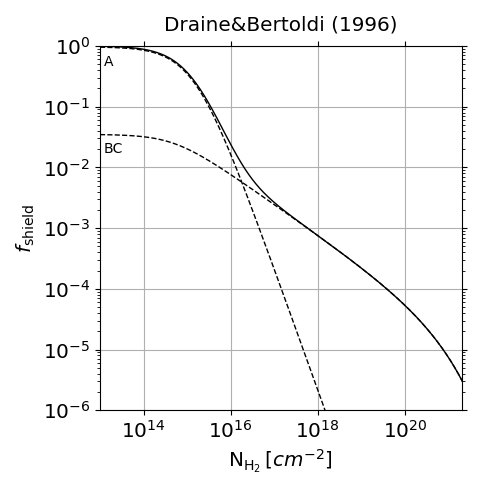
\includegraphics[width = 0.4\textwidth]{figure/H2/pomp/fshield.png}
    \caption{Fonction de shielding $f_\mathrm{shield}$ de $\mathrm{H}_2$ en fonction de la colonne densité $N(\mathrm{H}_2)$}
    \label{fig:H2:fshield}
\end{figure}


\subsubsection{Extinction par les grains}

Le champs de rayonnement calculé par le code ne prend pas en compte l'extinction par les grains. Approximation FGK. Je corrige le champs de rayonnement par $e^{-\tau_d}$ où $\tau_d = N_\mathrm{H}\sigma_d$ donné par \cite{SternbergLePetit2014} Eq 20. Ainsi, 

$$\chi^{'} = e^{-\tau_d
}\, f_{\mathrm{shield}}\, \chi$$


\subsection{Comparaison avec le code PDR de Meudon}

On récupère du code le taux de refroidissement $\Lambda_{\mathrm{PDR}}$ par la molécule $\mathrm{H}_2$ qui peut être positif ou négatif. Le taux prend en compte du chauffage par desexcitation collisionnelle et du refroidissement ro-vibrationelle (émission). Il ne prend pas en compte de la photodissociation (qui chauffe). On veut étudier le chauffage, on appelle $\Gamma_{\mathrm{PDR}}$ la partie négative du taux ($\Lambda_{\mathrm{PDR}} < 0$) et on le compare aux de chauffage nets.

\begin{equation}
    \begin{split}
        \Gamma_{\mathrm{Rollig} \, \mathrm{net}} &= \Gamma_{\mathrm{H}_2^\star} + \Lambda_{\mathrm{H}_2} \\ 
        \Gamma_{\mathrm{BS} \, \mathrm{net}} &=\Gamma_{\mathrm{H}_2 \, \mathrm{pump}} +  \Gamma_{\mathrm{H}_2 \, \mathrm{pd}} 
    \end{split}
\end{equation}

La figure \ref{fig:H2:GammaPDR} compare les taux de chauffages nets utilisant différentes prescriptions à celui calculé dans le code (en noir). Le chauffage calculé par Rollïg et de Bialy&Sternberg ont la même intensité en bord de nuage où la désexcitation collisionnelle est prédominante. 

L'approximation FGK est une méthode qui calcule le spectre du champs de rayonnements à travers le nuage qui prend en compte l'absorption dans le continuum et le carbone. Il prend également en compte l'écrantage de la molécule $\mathrm{H}_2$ (figure \ref{fig:H2:fgk} \cite{FGK}). 

\begin{figure}[h!]
    \centering
    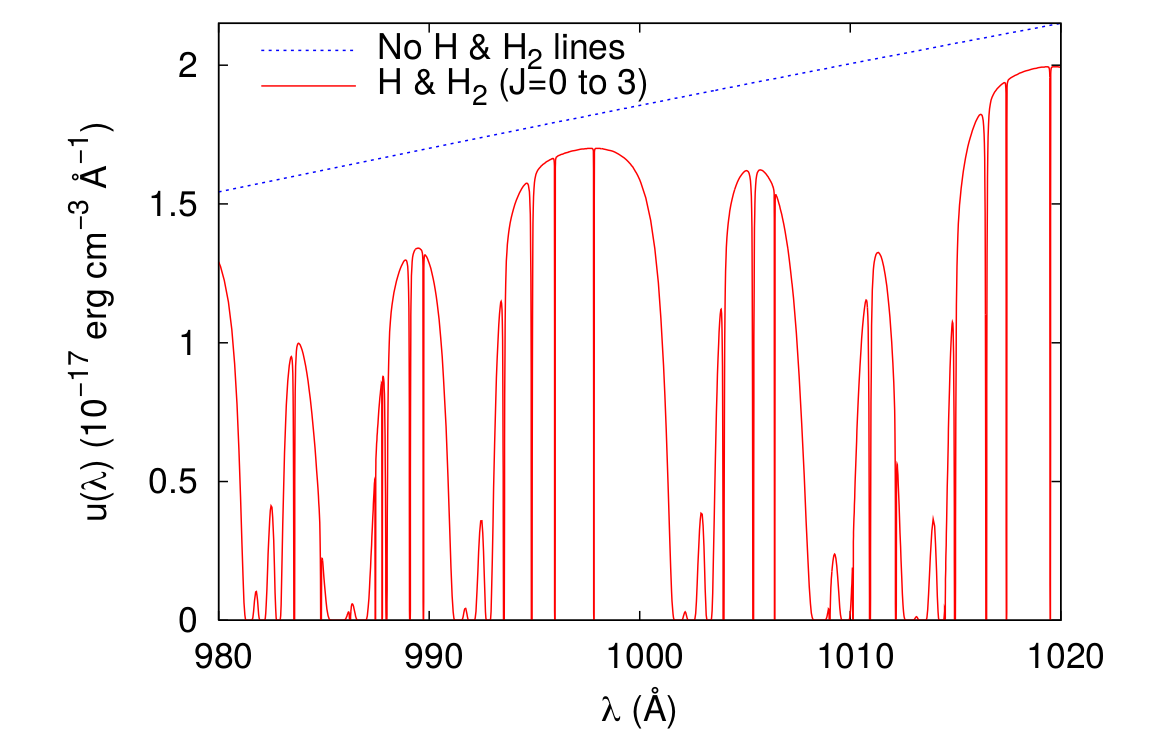
\includegraphics[width = 0.8\textwidth]{figure/H2/fgk.png}
    \caption{Densité d'énergie au sein d'un nuage à un $A_\mathrm{V}=0.5$. Les niveaux du $\mathrm{H}$ et de $\mathrm{H}_2$ absorbent certains photons sur certaines raies. A mesure que l'on s'enfonce dans le nuage beaucoup de matière se trouve sur la ligne de visée et les raies d'absroptions s'élargissent (voir optiquement épaisse Draine) \cite{FGK}}
    \label{fig:H2:fgk}
\end{figure}


\subsection{Prescription de Glover et Janev}

Dans la version \uncinq les taux de dissociation collisionelle de $\mathrm{H}_2$ via 

\begin{equation}
    \begin{array}{lcccccccl}
        \mathrm{H} & + & \mathrm{H}_2   & \rightarrow &\mathrm{H}  & + & \mathrm{H} & + & \mathrm{H} \\
        \mathrm{H}_2  & + & \mathrm{H}_2  & \rightarrow & \mathrm{H} & + &\mathrm{H}_2  & + & \mathrm{H} \\
    \end{array}
\end{equation}

sont calculé selon Janev (2008) (retrouver citation). On utilise une nouvelle version du code (\unsept) qui calcule aussi les taux de dissociation selon Janev : rien ne bouge. Les raies du $\mathrm{H}_2$ et du $\mathrm{CO}$ sont les mêmes et le profils de température aussi. On utilise dorénavant pour cette étude la version \unsept. On compare la prescription de Glover à celle de Janev et on remarque plusieurs choses. Tout d'abord les raies d'émissions de $\mathrm{H}_2$ et $\mathrm{CO}$ sont augmentées (\autoref{figu:H2:..}). De plus le profil de température avec la nouvelle prescription (Glover) est modifié un tout petit peu au au bord (+100K) et un peu à l'entrée du nuage moléculaire (+400K) (\autoref{fig:H2:JanevGlover:emiss}). L'augmentation de la température à l'entrée du nuage moléculaire ($A_\mathrm{V} = 0.8$) provient du chauffage par exothermicité des réactions chimiques qui devient majeure (jusqu'à $50\%$ du chauffage total). Janev a tendance à surestimer les taux de dissociation qui sont toutes deux des réactions endothermiques et qui ont des efficacités de refroidissement les plus importantes. Les taux calculé par Glover réduisent leur refroidissement globale sur le nuage ce qui le chauffe. \newline 


\begin{figure}[h!]
    \centering
    \begin{subfigure}[t]{0.45\textwidth} % "0.45" donne ici la largeur de l'image
        \centering 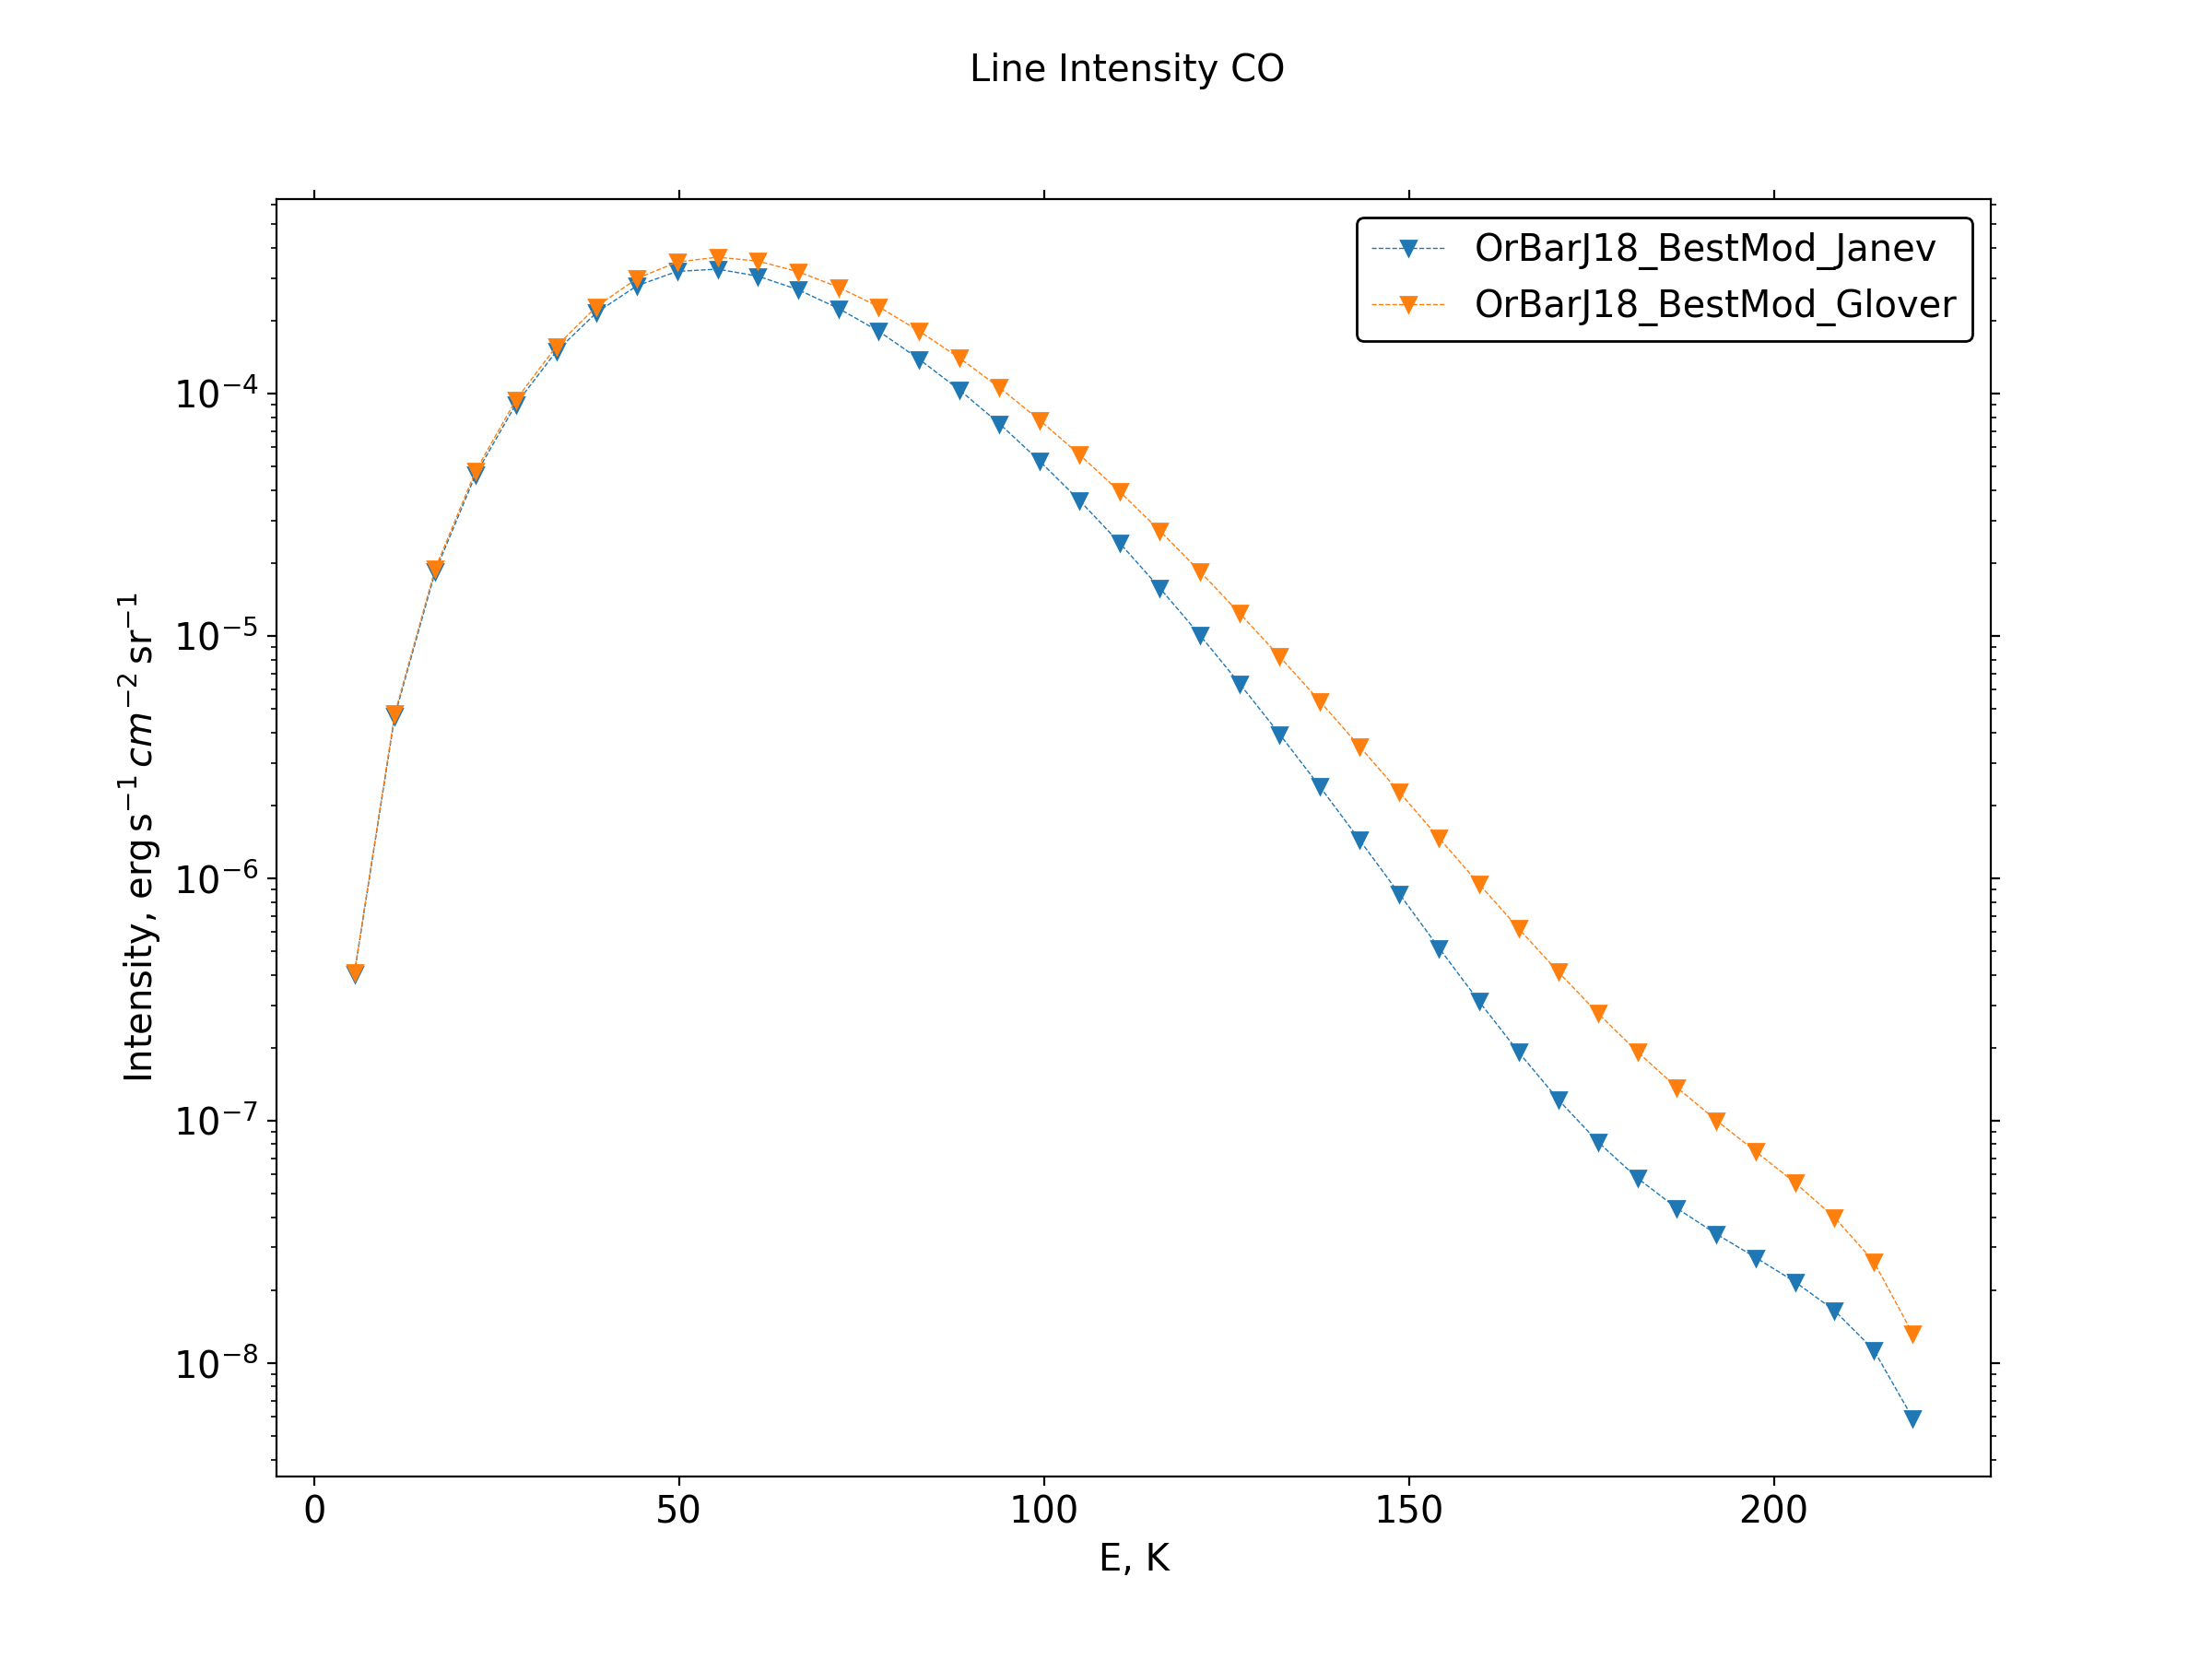
\includegraphics[trim = {0 0 0 1.5cm},clip,width=1\textwidth]{figure/H2/JanevGlover/I_comp_CO.png}
        \caption{Spectre $\mathrm{H}_2$}
    \end{subfigure}
    ~ 
    \begin{subfigure}[t]{0.45\textwidth}
        \centering 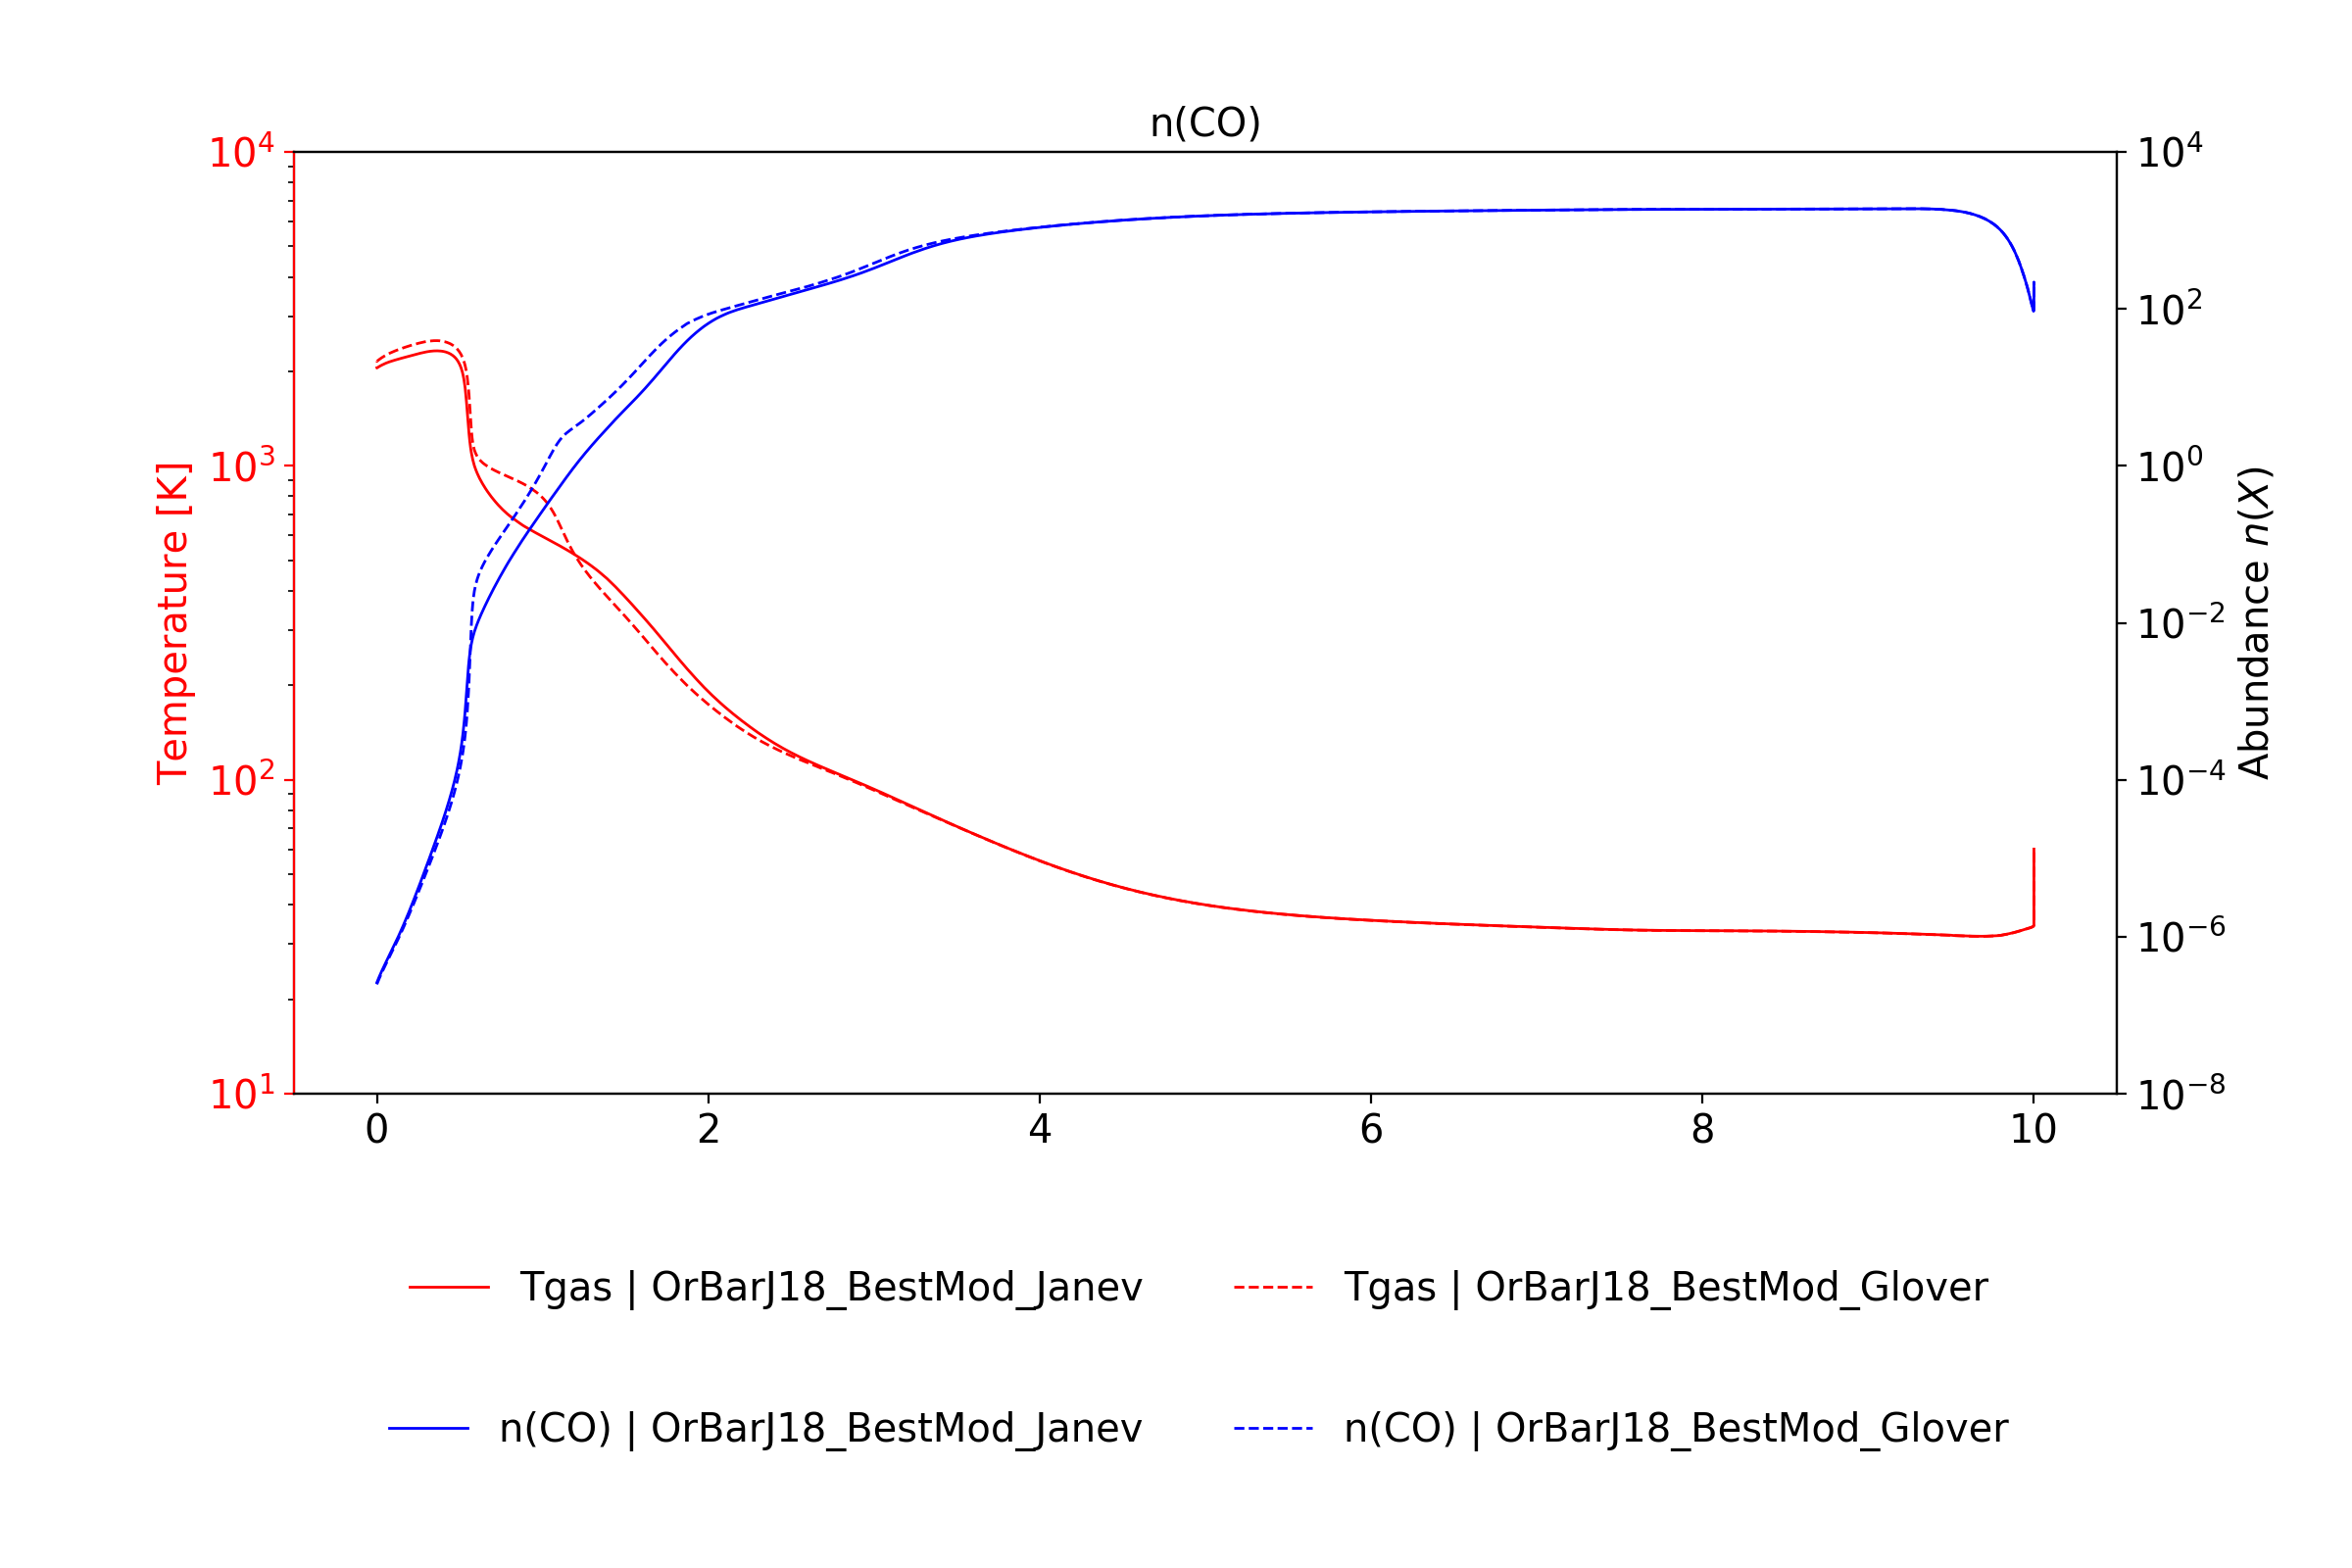
\includegraphics[trim = {0 0 0 1.5cm},clip,width=1\textwidth]{figure/H2/JanevGlover/nT_comp_CO.png}
        \caption{Profil de densité et température de $\mathrm{H}_2$}
    \end{subfigure}

    \centering
    \begin{subfigure}[t]{0.45\textwidth} % "0.45" donne ici la largeur de l'image
        \centering 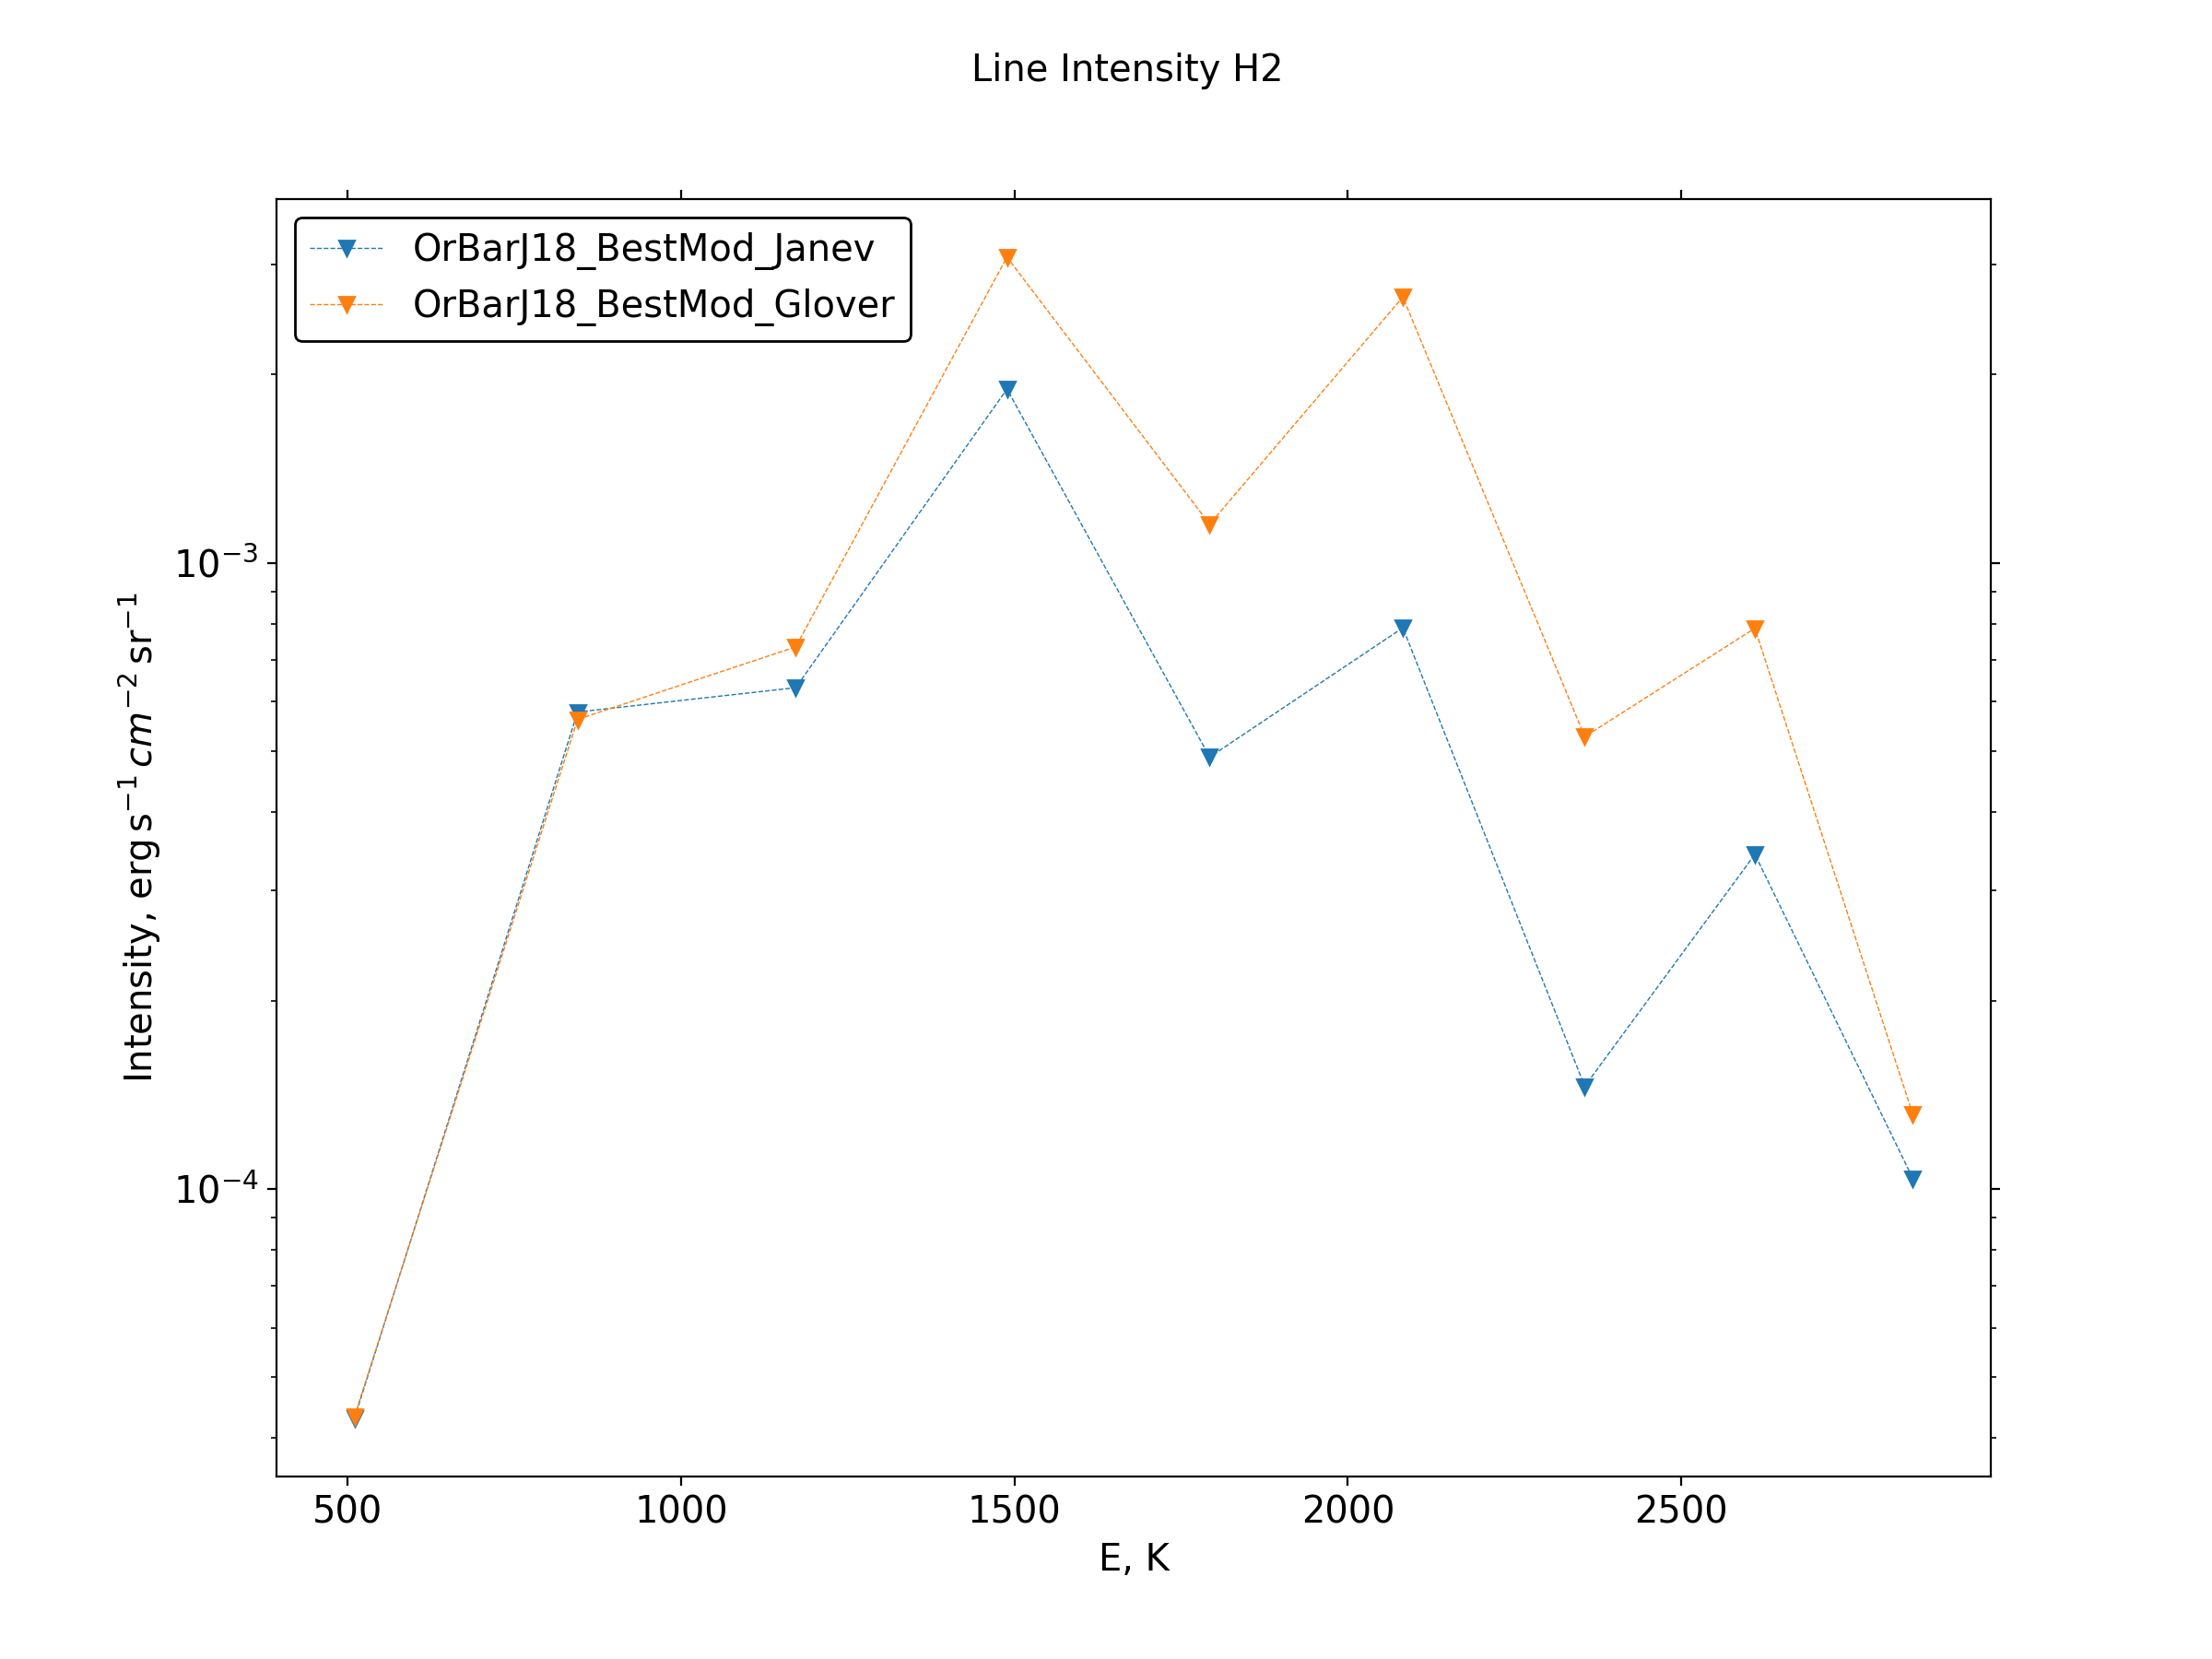
\includegraphics[trim = {0 0 0 1.5cm},clip,width=1\textwidth]{figure/H2/JanevGlover/I_comp_H2.png}
        \caption{Spectre de $\mathrm{CO}$}
    \end{subfigure}
    ~ 
    \begin{subfigure}[t]{0.45\textwidth}
        \centering 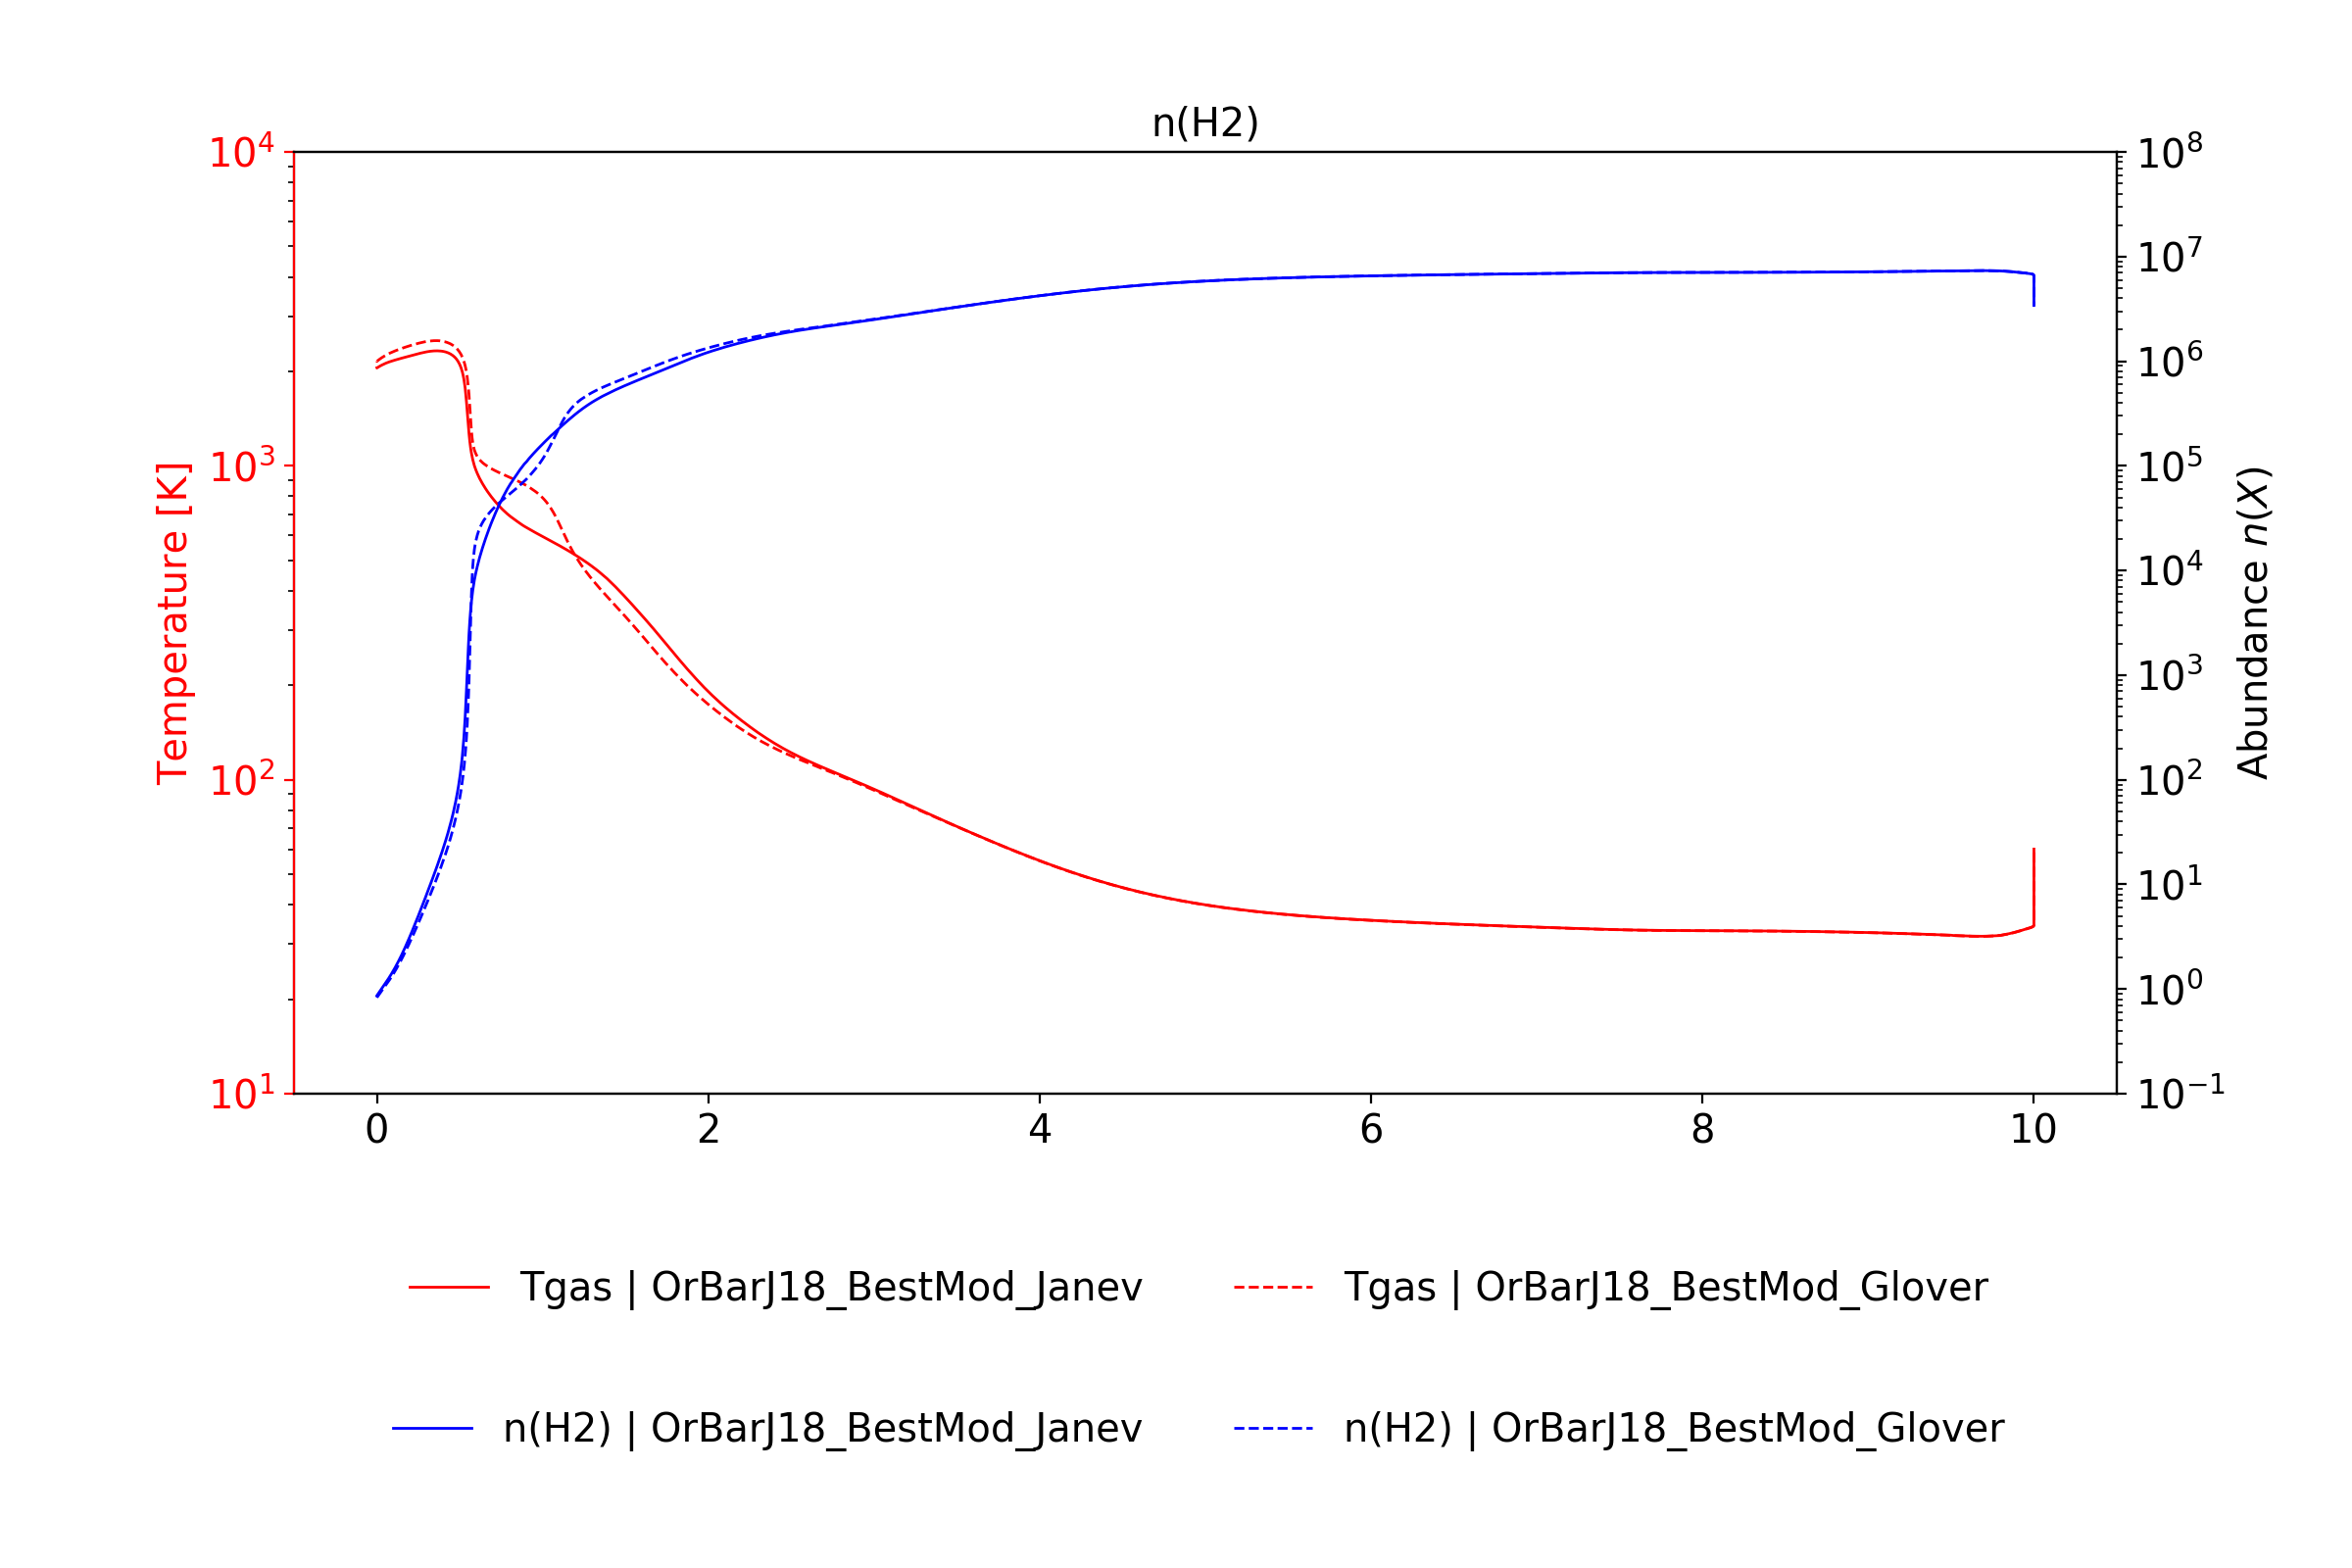
\includegraphics[trim = {0 0 0 1.5cm},clip,width=1\textwidth]{figure/H2/JanevGlover/nT_comp_H2.png}
        \caption{Profil de densité et température de $\mathrm{CO}$}
    \end{subfigure}
    \caption{Impact des prescriptions de Janev et Glover sur les raies d'émissions des traceurs $\mathrm{H}_2$ et $\mathrm{CO}$}
    \label{fig:H2:JanevGlover:emiss}
\end{figure}


Néanmoins on connaît mal la proportion effective qui chauffe le gaz par exothermicité alors que l'on compte sur elle pour exciter nos raies. Il faut reprendre l'étude sur l'exothermicité des réactions chimiques et jouer sur cette prescription. \newline 

On cherche à visualiser l'impact des nouveaux calculs des niveaux de $\mathrm{H}_2$ sur les raies. On l'a calculé dans le cas de Janev et Glover mais l'on montre seulement la prescription de Glover qui est la plus importante (\autoref{fig:H2:GloverBossion:emiss})

On se rend compte que l'impact est minime alors que le travail pour calculer ces niveaux est lourd. Au moins on sait que connaître précisément les niveaux de $\mathrm{H}_2$ n'est pas décisif dans l'interprétation des spectres d'émissions. Il faut explorer d'autres possibilités. 

\begin{figure}[h!]
    \centering
    \begin{subfigure}[t]{0.45\textwidth} % "0.45" donne ici la largeur de l'image
        \centering 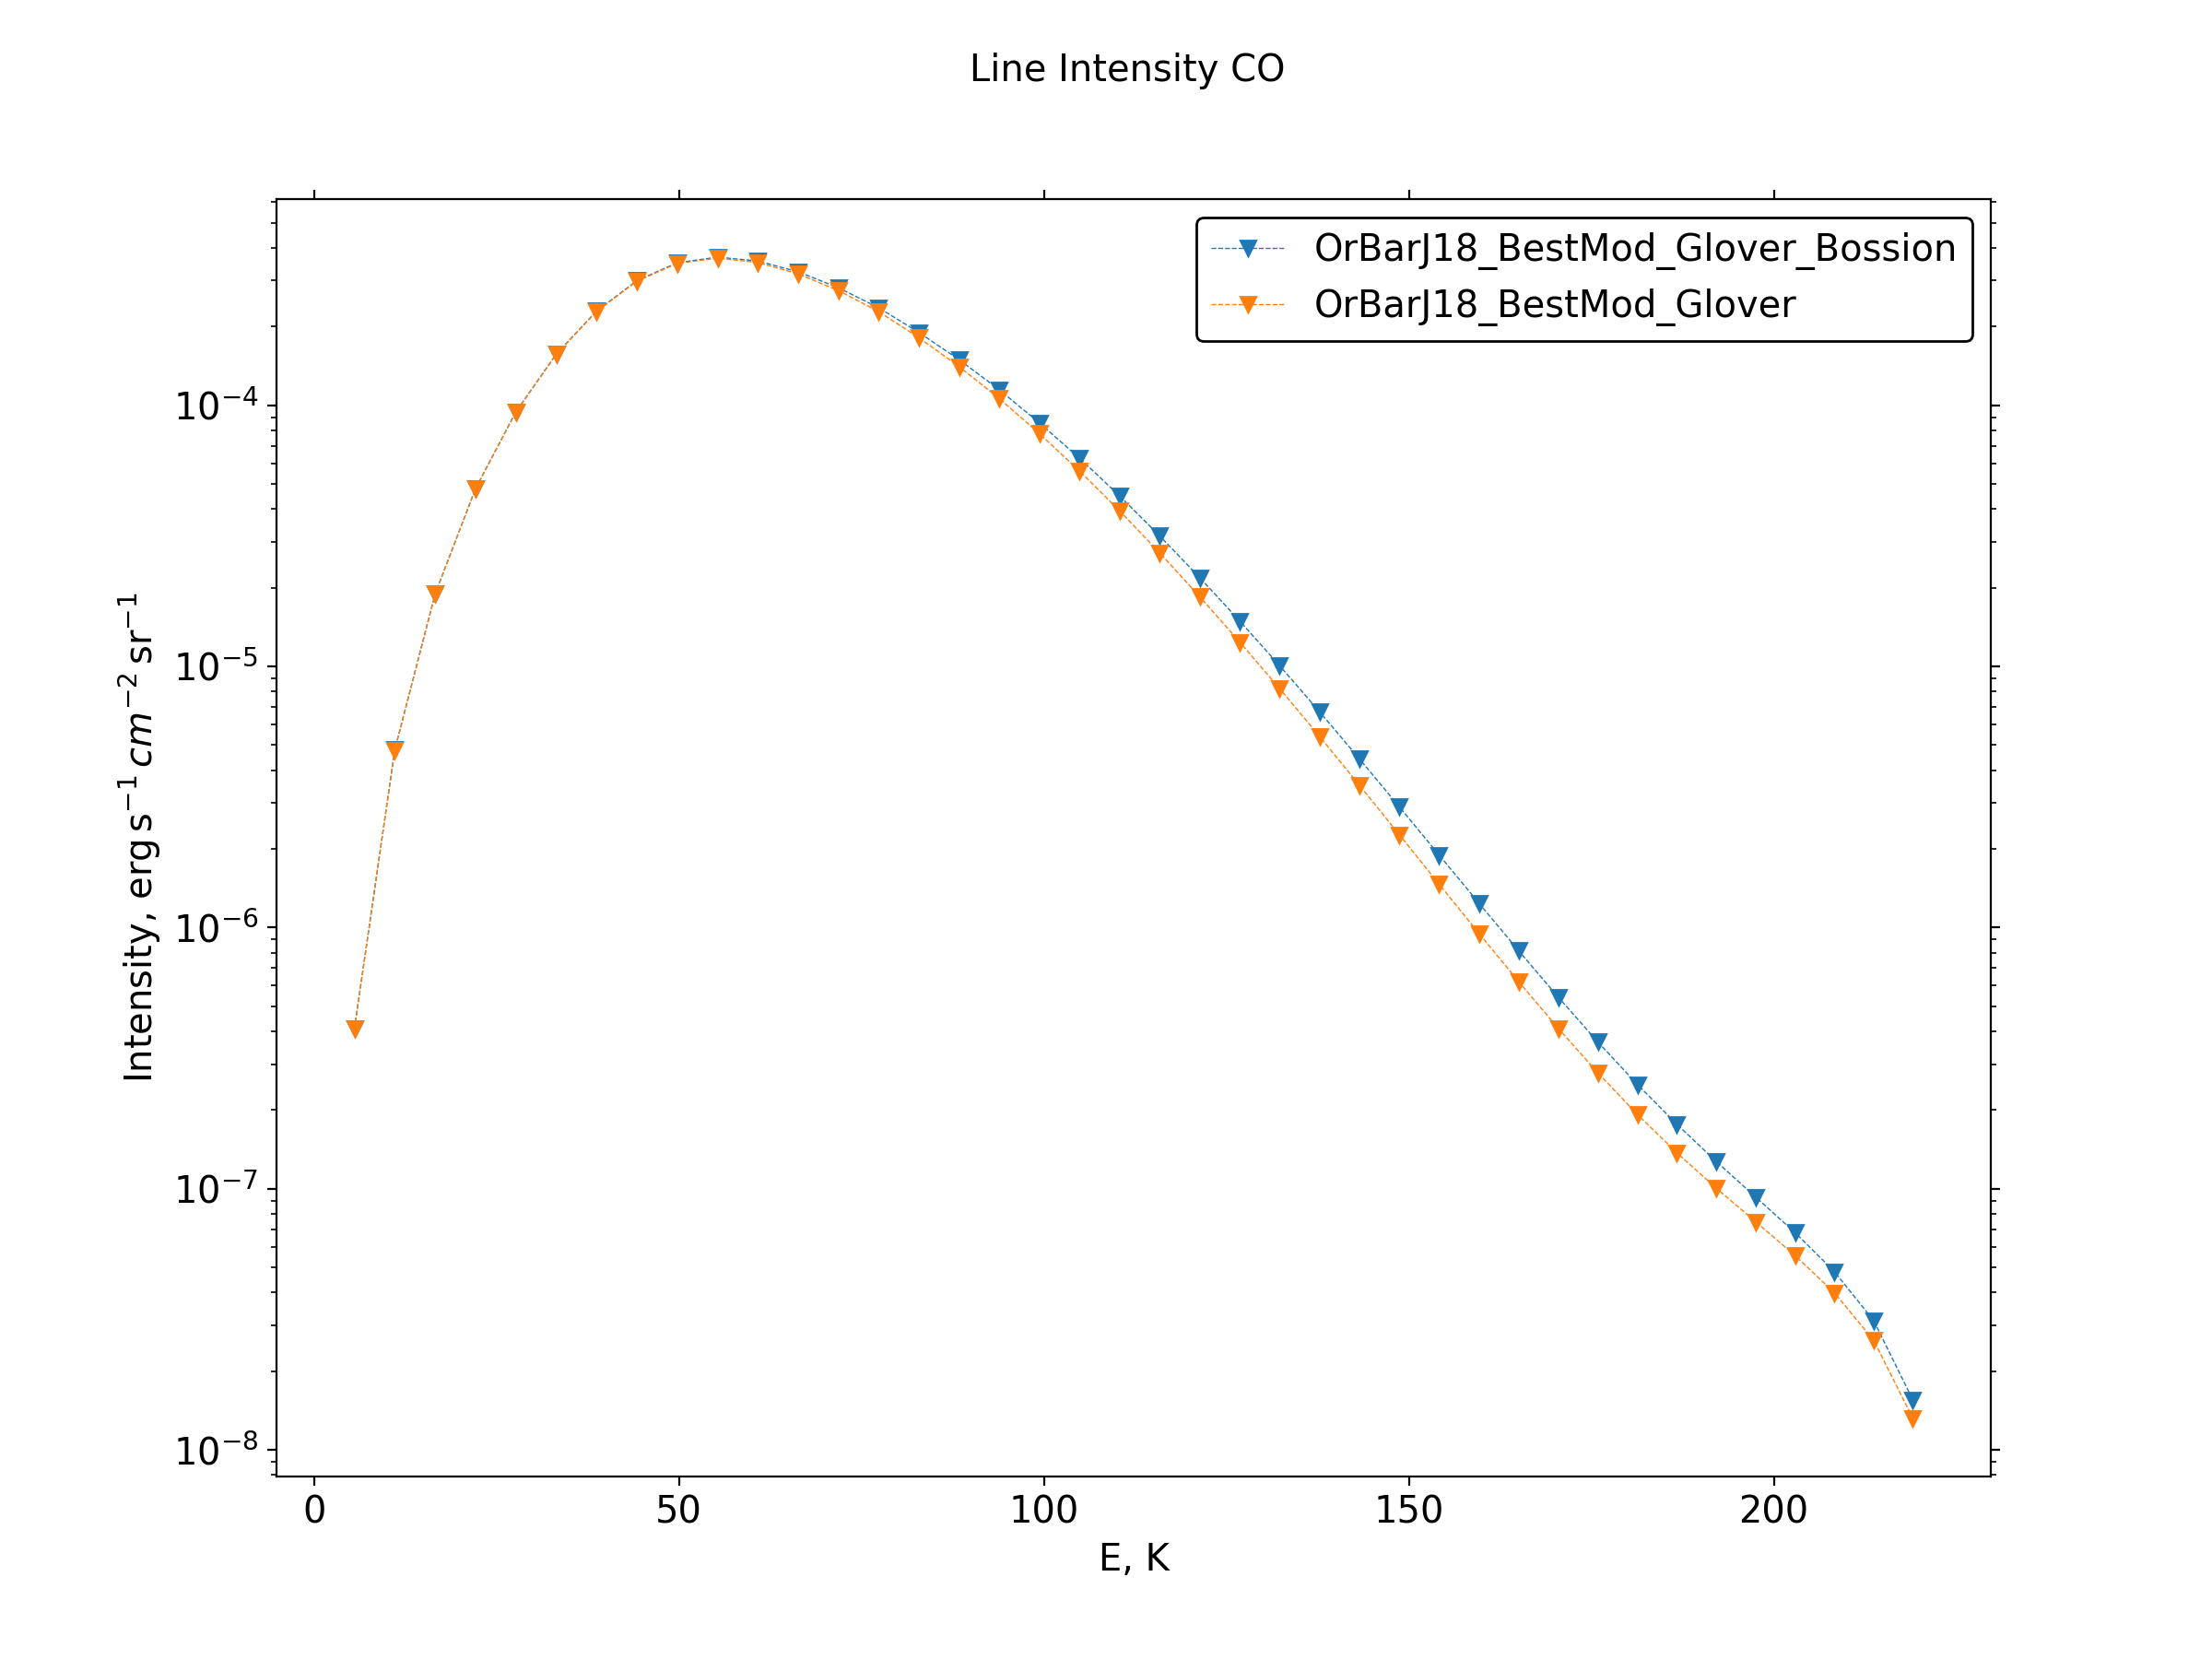
\includegraphics[trim = {0 0 0 1.5cm},clip,width=1\textwidth]{figure/H2/GloverBossion/I_comp_CO.png}
        \caption{Spectre $\mathrm{H}_2$}
    \end{subfigure}
    ~ 
    \begin{subfigure}[t]{0.45\textwidth}
        \centering 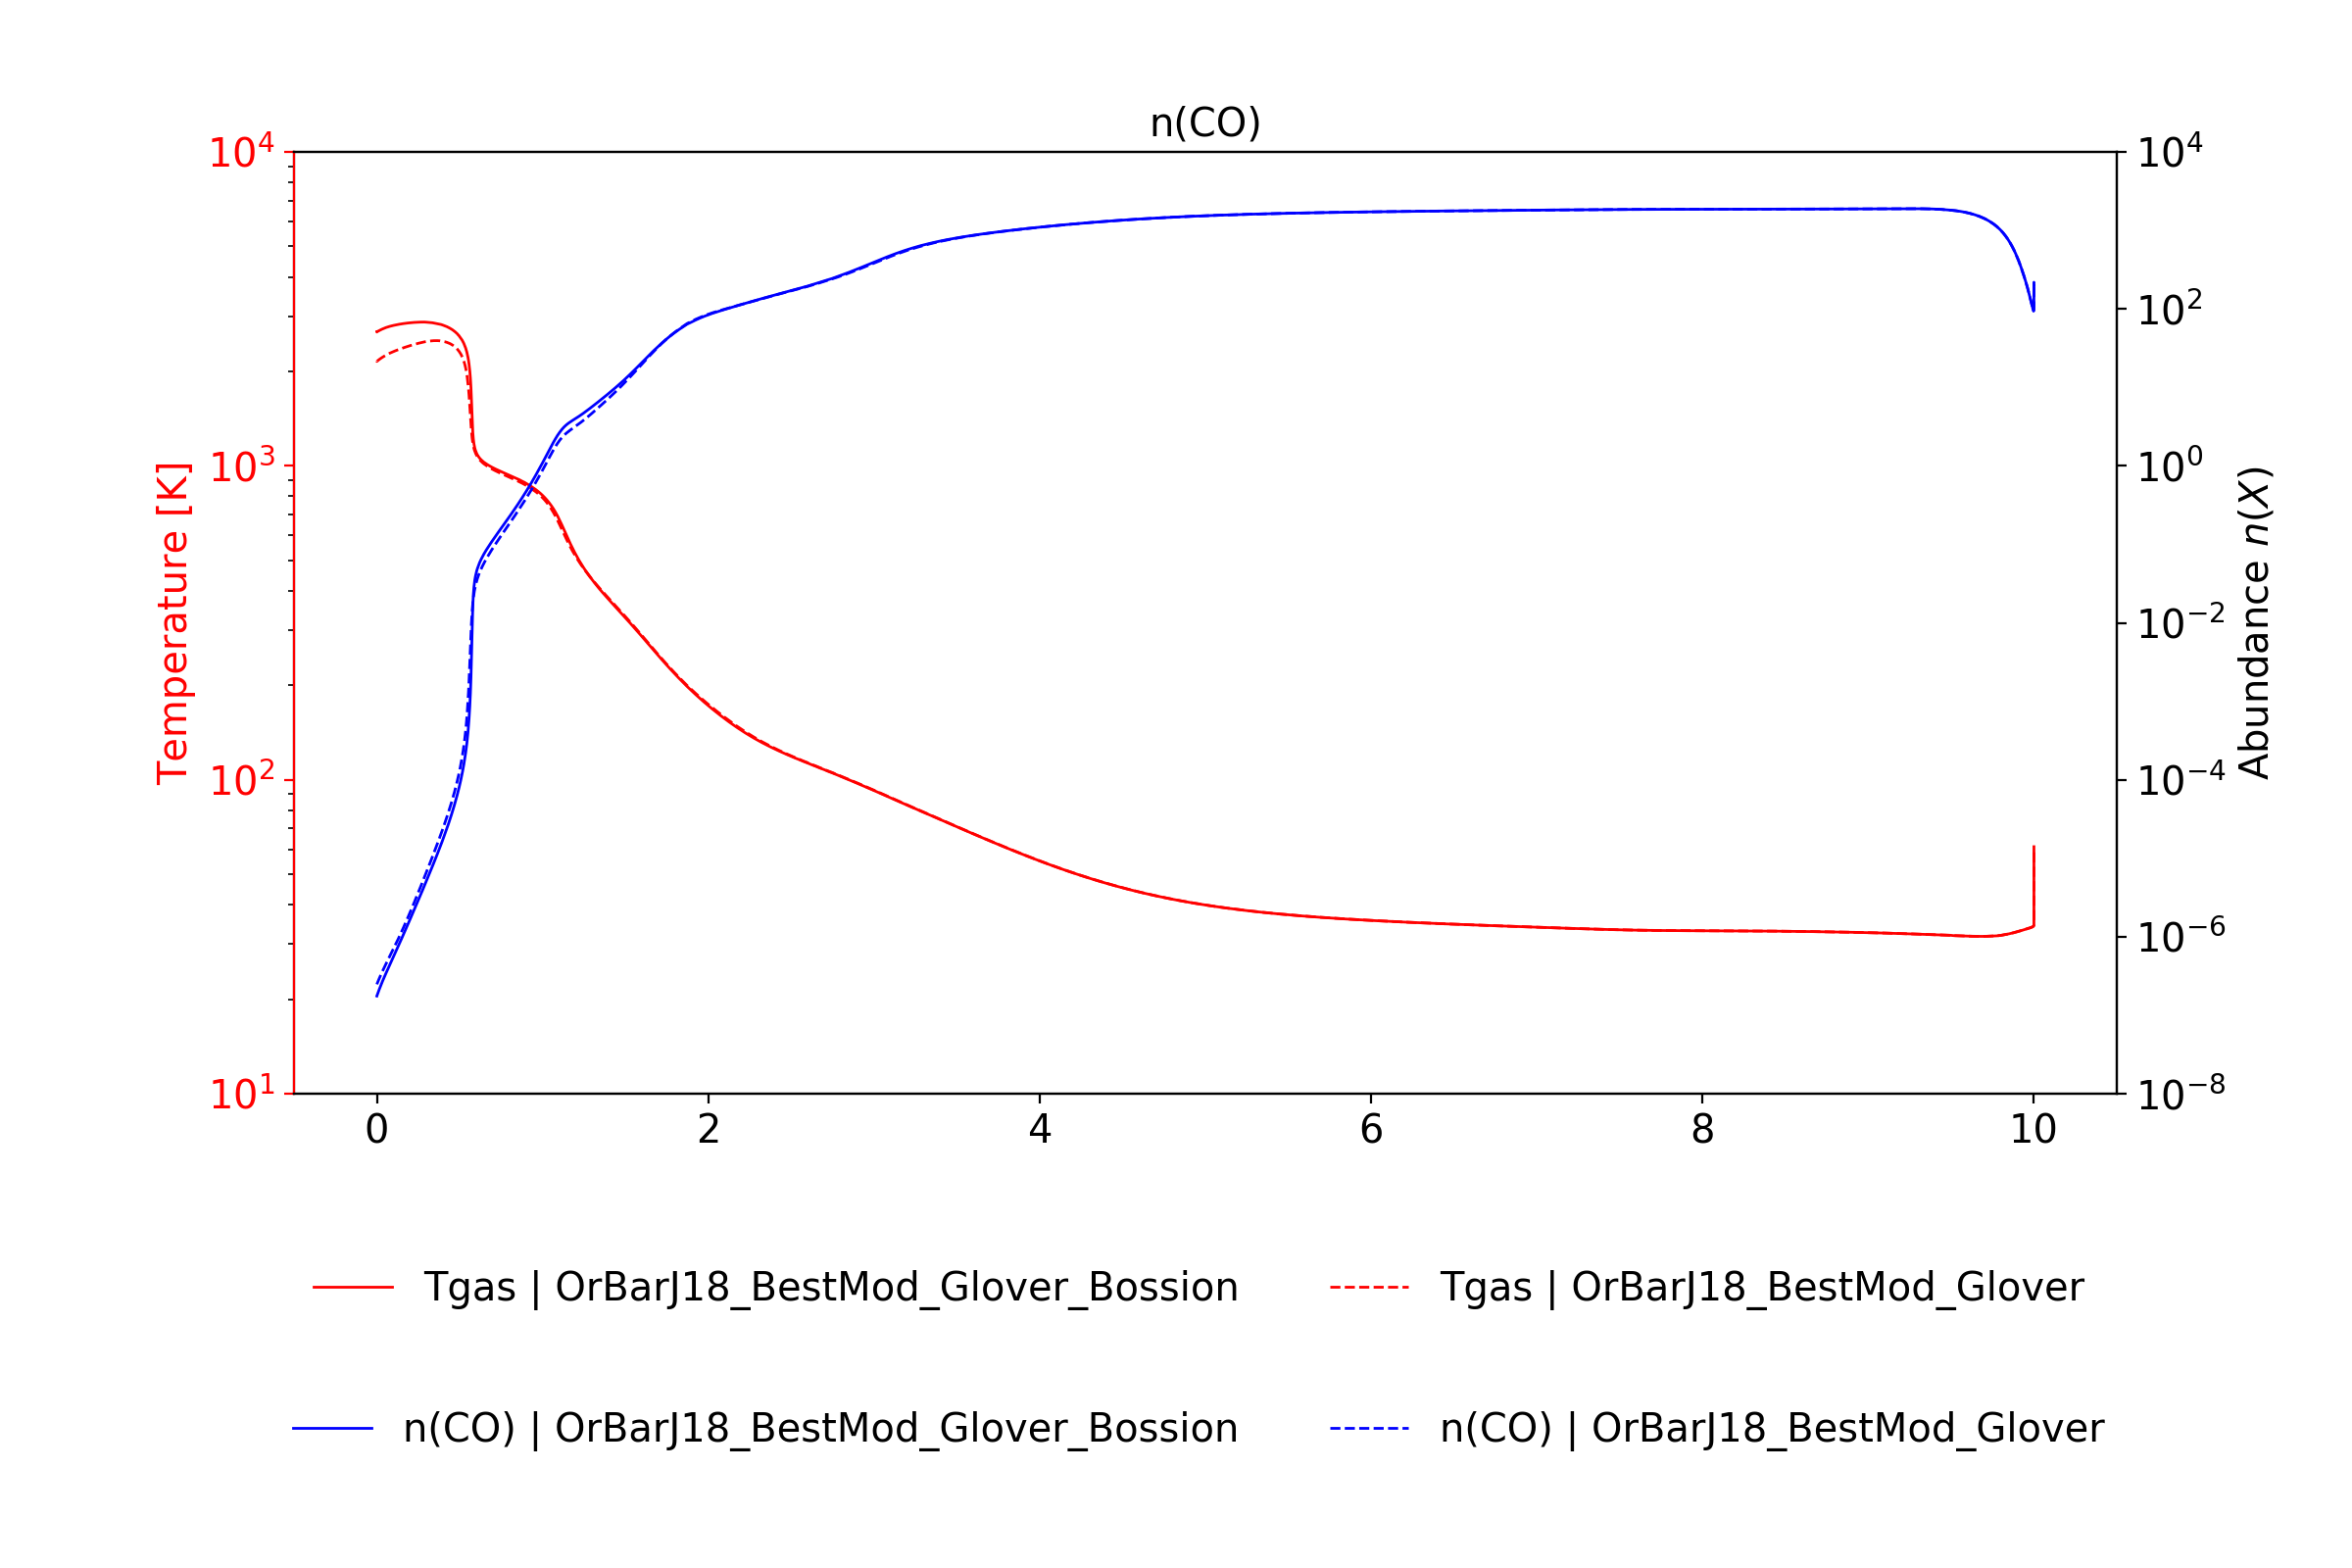
\includegraphics[trim = {0 0 0 1.5cm},clip,width=1\textwidth]{figure/H2/GloverBossion/nT_comp_CO.png}
        \caption{Profil de densité et température de $\mathrm{H}_2$}
    \end{subfigure}

    \centering
    \begin{subfigure}[t]{0.45\textwidth} % "0.45" donne ici la largeur de l'image
        \centering 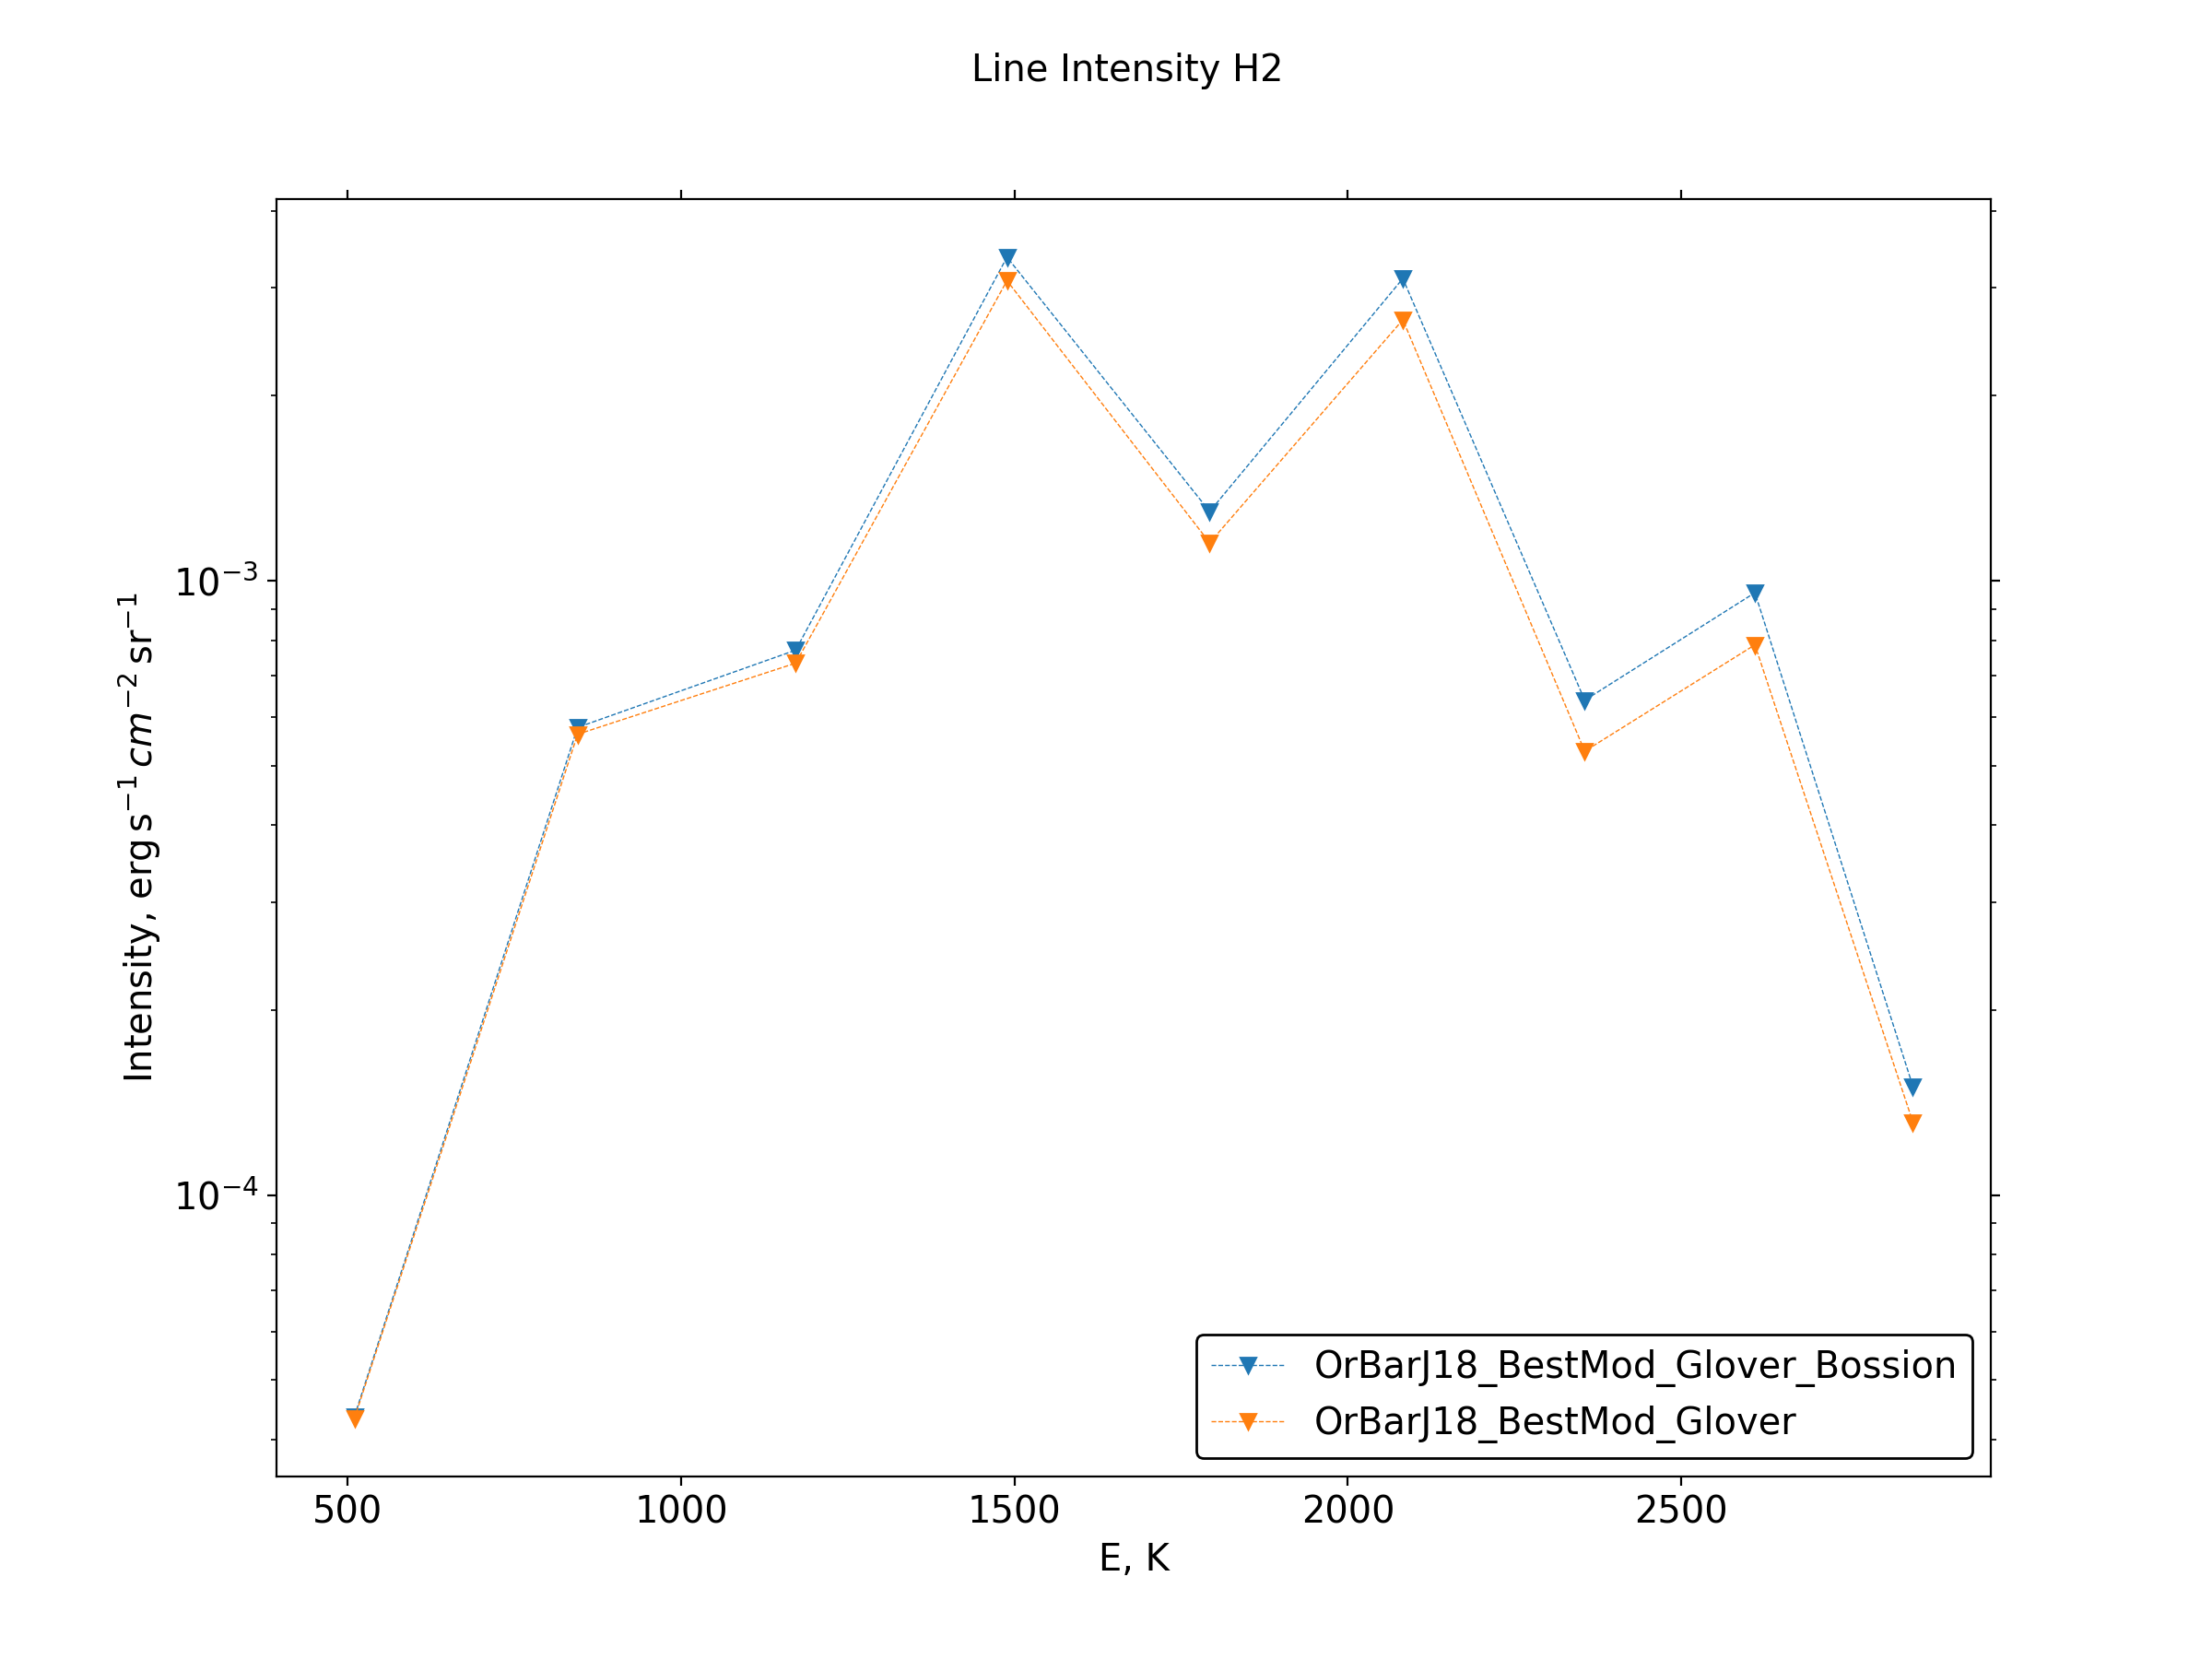
\includegraphics[trim = {0 0 0 1.5cm},clip,width=1\textwidth]{figure/H2/GloverBossion/I_comp_H2.png}
        \caption{Spectre de $\mathrm{CO}$}
    \end{subfigure}
    ~ 
    \begin{subfigure}[t]{0.45\textwidth}
        \centering 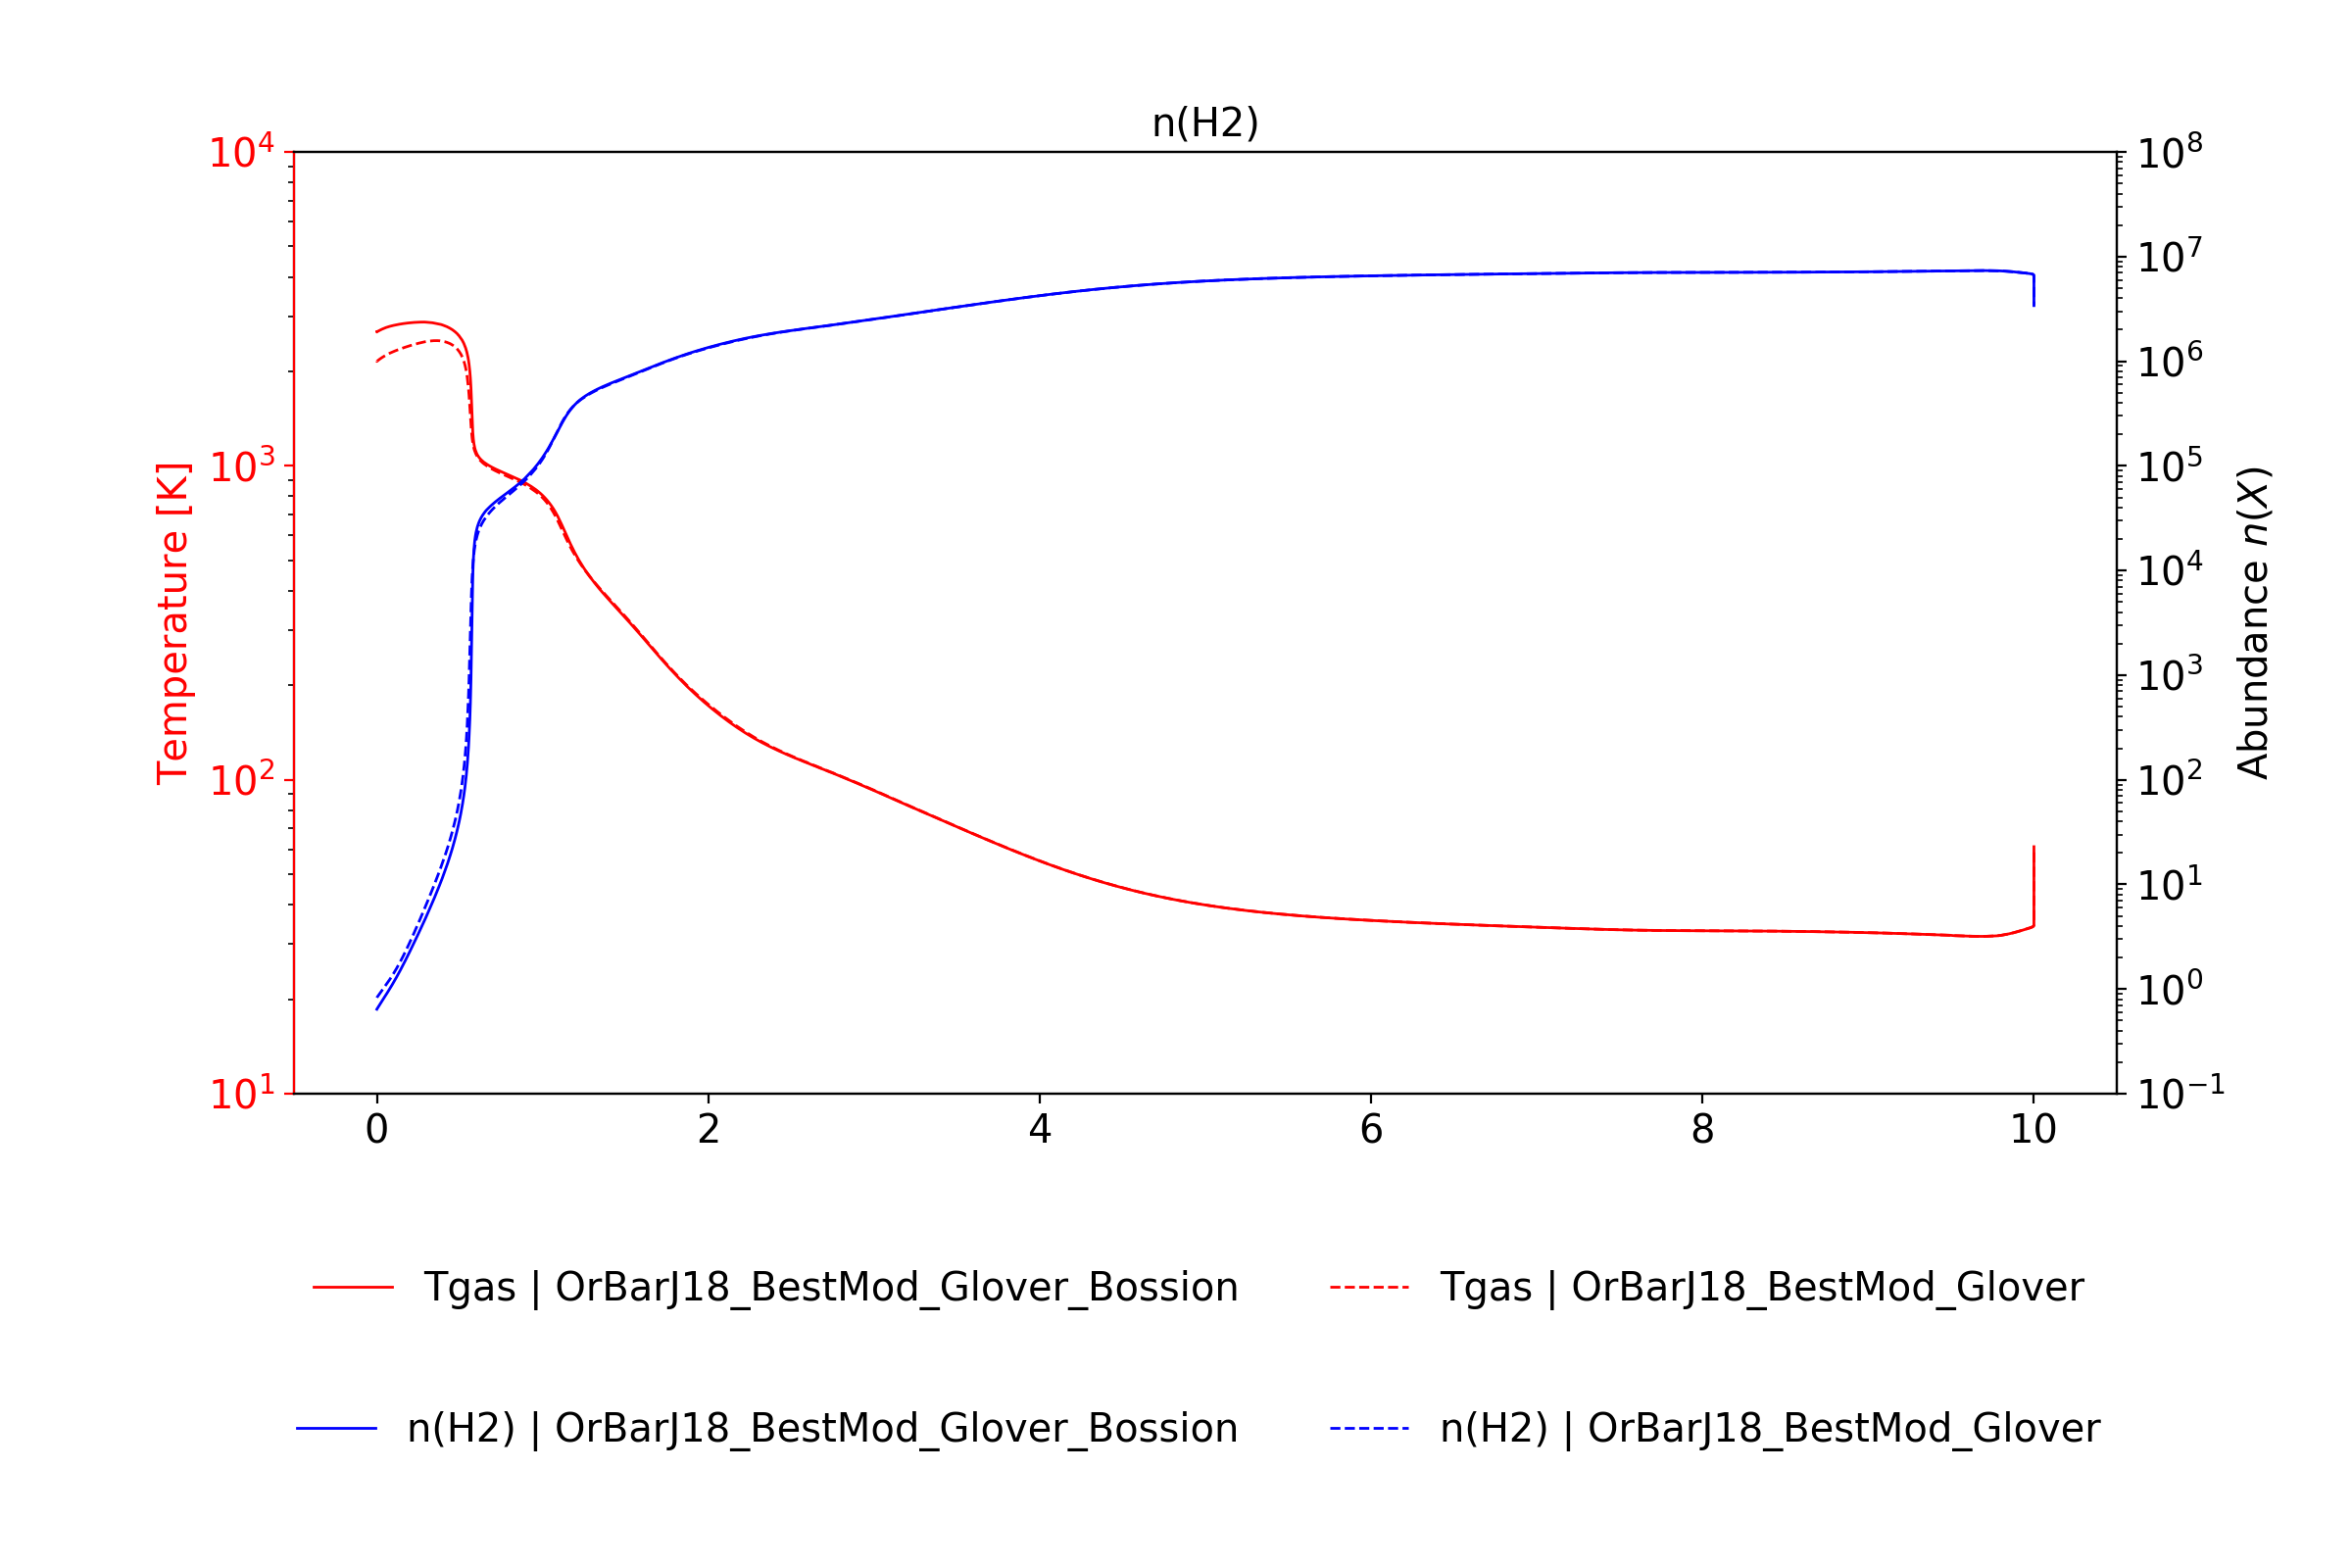
\includegraphics[trim = {0 0 0 1.5cm},clip,width=1\textwidth]{figure/H2/GloverBossion/nT_comp_H2.png}
        \caption{Profil de densité et température de $\mathrm{CO}$}
    \end{subfigure}
    \caption{Impact des nouveaux calculs classiques (Bossion) avec la prescription de Glover sur les raies d'émissions des traceurs $\mathrm{H}_2$ et $\mathrm{CO}$}
    \label{fig:H2:GloverBossion:emiss}
\end{figure}


